\chapter{Simile}
\label{chap:simile}
In this chapter we present the our approach that seizes Continuous Integration process in order to recommend similar components that are being developed in a software project. The idea of integrating CI and Software reuse emerged with the following research question: \emph{How can code search engines be best married with CI?}. The idea was to find a way where a team could seize the continuous integration process in order to find similar components to the components they are developing. Thus they would be able to reuse instead of implementing them from scratch reducing development time and costs. As an attempt to answer the question we implemented a tool (proof of concept) called Simile. This tool analyses the source code and extract information needed to find similar components.

Following the usage scenario explained previously in section \ref{usage-scenario}, we will describe how our proposed approach works:

\begin{figure}[H]
	\centering
    \includegraphics[width=0.8\textwidth]{grafiken/simile-approach}
    \caption{Simile approach}
    \label{fig:simile-01}
\end{figure}

In the first step (figure \ref{fig:simile-01} - 1) the developer commits code to its local VCS. Then when the developer decides to push changes to the remote repository, the CI server is triggered (figure \ref{fig:simile-01} - 2). In the next step (figure \ref{fig:simile-01} - 3), Simile will analyse the code and extract information such as interfaces signatures and test classes. This information will be sent to SOCORA (figure \ref{fig:simile-01} - 4) in order to find similar components. Then it will return a ranked list of similar components. Simile will receive this information and send this list to the developers by email (figure \ref{fig:simile-01} - 5).

The main objective of Simile is to help the team to find similar components so they would be able to reuse them. Thus they would reduce time development and costs through reuse components that are already tested and ready to work.

In the following sections we will explain in details how Simile was implemented. Then we will detail how we integrate Simile into Continuous Integration server (Jenkins). After that we will explain how we integrate Simile and SOCORA for searching for similar components.

\section{Implementation}
In this section we will detail how the prototype was developed and the technologies used. First we will start explaining the Simile service which is the starting point of the whole process about cloning the project, analyse code, search components and send result. Then we will continue with the  HTTP controller which receives the Git repository of the project to be analysed, the specific branch of the repository, and the email where the result will be sent. Then we will explain the Cloner object which is in charge of cloning the project locally. After that, we will explain how the tool analyses the code and extracts the interface signatures and test classes which will be used to make the requests to SOCORA. Next we will describe how we receive the result from SOCORA. Finally we will explain how we handle the result from the previous step and build the email that will be sent to user.

\textbf{NOTE: The code snippet shown in the following subsections has been cleaned and it does not represent the source code. To see the source code with all the details, please refer to the appendix \ref{append:simile-code} or to the CD attached to this work.}

\subsection{Simile}
The class Simile.java [\ref{Simile.java}] is a Spring service which contains only one method, \emph{searchForComponents}. This methods receives four parameters, repo, branch, folder, and recipient. \emph{repo} represents the Git repository of the project to be analysed. \emph{branch} is the branch of the Git repository (optional). \emph{folder} represents the name of the folder where the project will be cloned. Finally \emph{recipient} is the email where Simile will send the result. Listing \ref{searchForComponents} represents the method.

\lstinputlisting[
  language=Java, numbers=left, firstnumber=1, breaklines=true, 
  basicstyle=\footnotesize,
  numberstyle=\tiny,
  caption={Method searchForComponents of Simile.java},
  captionpos=b,
  label=searchForComponents
]
{code/Simile-searchForComponents.txt}

First, it clones the project in the server by calling the method \emph{cloneRepository} of Cloner [\ref{Cloner.java}]. Then it analyses the Java main code of the project cloned and the test classes. When it analyses the code it extracts the interface signatures and the test classes, we explain how it does this process in section \ref{code-analysis}. With the result of the previous step, we make the requests to SOCORA to search for similar components.

It is important to notice that this method is asynchronous by the Java annotation \emph{@Async}. This allows us to run this method many times in parallel (configured in SimileApplication.java \ref{SimileApplication.java}).

\subsection{Cloner}
\label{simile:cloner}
The class Cloner.java [\ref{Cloner.java}] is in charged of cloning the project in a local directory. The listing \ref{cloneRepository} represents the method \emph{cloneRepository}.

\lstinputlisting[
  language=Java, numbers=left, firstnumber=1, breaklines=true, 
  basicstyle=\footnotesize,
  numberstyle=\tiny,
  caption={Method cloneRepository of Cloner.java},
  captionpos=b,
  label=cloneRepository
]
{code/Cloner-cloneRepository.txt}

This method runs the command \emph{git clone} with the parameters \emph{repo}, \emph{branch}, and \emph{folder}. The command is built by the private method \emph{setCommand}. After running the command, the project is cloned locally under the folder with given \emph{folder} name.

\subsection{Interface signature and test class extraction}
\label{simile:code-analysis}
In this section we will explain how Simile explores the project cloned and extracts the interface signatures and test classes that will be sent to SOCORA to search for similar components.

After the project is cloned locally by the Cloner (\ref{simile:cloner}), Simile goes through the code and extract interface signatures of each class, and test classes. The signatures extracted are transformed into Merobase Query Language (MQL) notation, and the test classes are extracted as is. The snipped code \ref{handler} shows how the interface signatures are extracted and transformed into MQL. For extracting test classes the principle is the same, the difference is that we differentiate a Test class from another Java file if it contains the annotation \emph{@Test}.

\lstinputlisting[
  language=Java, numbers=left, firstnumber=1, breaklines=true, 
  basicstyle=\footnotesize,
  numberstyle=\tiny,
  caption={Method handle of JavaClassHandler.java},
  captionpos=b,
  label=handler
]
{code/JavaClassHandler-handle.txt}

In the class JavaClassVisitor.java we can see how Simile differentiate between a normal Java class and a test class. It implements the methods \emph{visit} for a \emph{ClassOrInterfaceDeclaration} and for a \emph{MethodDeclaration} object of the abstract class VoidVisitorAdapter. The listing \ref{visit} show the implementation of these methods.

\lstinputlisting[
  language=Java, numbers=left, firstnumber=1, breaklines=true, 
  basicstyle=\footnotesize,
  numberstyle=\tiny,
  caption={Implementation of methods \emph{visit} of VoidVisitorAdapter in JavaClassVisitor.java},
  captionpos=b,
  label=visit
]
{code/JavaClassVisitor-visit.txt}

To analyses the code we use the library Java Parser \footnote{\url{https://github.com/javaparser/javaparser} (accessed: 06.02.2017).}. This library parses Java code and creates an AST \footnote{Abstract syntax tree (AST): abstract syntax tree (AST), or just syntax tree, is a tree representation of the abstract syntactic structure of source code written in a programming language.}, which records the source code structure, javadoc and comments. Moreover, the library allows to change the AST nodes or create new ones to modify the source code.

\subsection{SOCORA Integration}
\label{socora-integration}
Our prototype uses SOCORA to search for components. After extracting the interface signatures and test classes from the project, Simile make requests to SOCORA using this information. SOCORA then searches for similar components using Merobase and ranks the candidates using non-functional requirements. Once it is done, SOCORA sends the result back to Simile.

Simile communicates with SOCORA by making HTTP requests using the interface signatures and the test classes extracted. The following snippet of code show how Simile is making the request for SOCORA \ref{textualSearchComponent}.

\lstinputlisting[
  language=Java, numbers=left, firstnumber=1, breaklines=true, 
  basicstyle=\footnotesize,
  numberstyle=\tiny,
  caption={Method textualSearchComponent of SocoraRequester.java},
  captionpos=b,
  label=textualSearchComponent
]
{code/SocoraRequester-textualSearchComponent.txt}

The class in charge of making the request to SOCORA is \emph{SocoraRequester.java}[\ref{SocoraRequester.java}]. The method \emph{searchComponent} receives two parameters, \emph{queries} which represents the interface signatures or the test classes, and \emph{searchType} which represents the type of search (i.e. test driven search, interface driven search or textual search (default)). The snippet of code \ref{searchComponent} represent the method \emph{searchComponent}.

\lstinputlisting[
  language=Java, numbers=left, firstnumber=1, breaklines=true, 
  basicstyle=\footnotesize,
  numberstyle=\tiny,
  caption={Method searchComponent of SocoraRequester.java},
  captionpos=b,
  label=searchComponent
]
{code/SocoraRequester-searchComponent.txt}

When SOCORA responses with the list of components found they are sent by email to developers. This action is done in the methods \emph{textualSearchComponent} or \emph{testDrivenSearchComponent} using the service EmailSender [\ref{EmailSender.java}].

\subsection{Email result}
After making the requests to SOCORA \ref{socora-integration}, it will response with the candidate components found. Simile receives the list of candidates, it extracts the candidates from the response, builds the email, and sends it to the recipient. For textual search results, the method \emph{processTemplateTextualSearchResult} is in charge of interpreting the result and process the email's template before it is sent. For test-driven results, the method \emph{processTemplateTestDrivenSearchResult} is in charge of interpreting the result and process the email's template before it is sent. The listing \ref{resultInterpretation} show this method.

\lstinputlisting[
  language=Java, numbers=left, firstnumber=1, breaklines=true, 
  basicstyle=\footnotesize,
  numberstyle=\tiny,
  caption={Methods \emph{processTemplateTextualSearchResult} and \emph{processTemplateTestDrivenSearchResult} of SocoraRequester.java},
  captionpos=b,
  label=resultInterpretation
]
{code/SocoraRequester-responseInterpretation.txt}

After the email's body is generated by using the template and the java objects, it is sent to the recipient. For building the email we use FreeMarker \footnote{\url{http://freemarker.org/} (accessed: 16.02.2017)}, which is a template engine which generates text output (HTML web pages, e-mails, configuration files, source code, etc.) based on templates and changing data. The figures \ref{fig:email-01} and \ref{fig:email-02} show the email with the result of a textual search and a test-driven search respectively.

\begin{figure}[H]
	\centering
    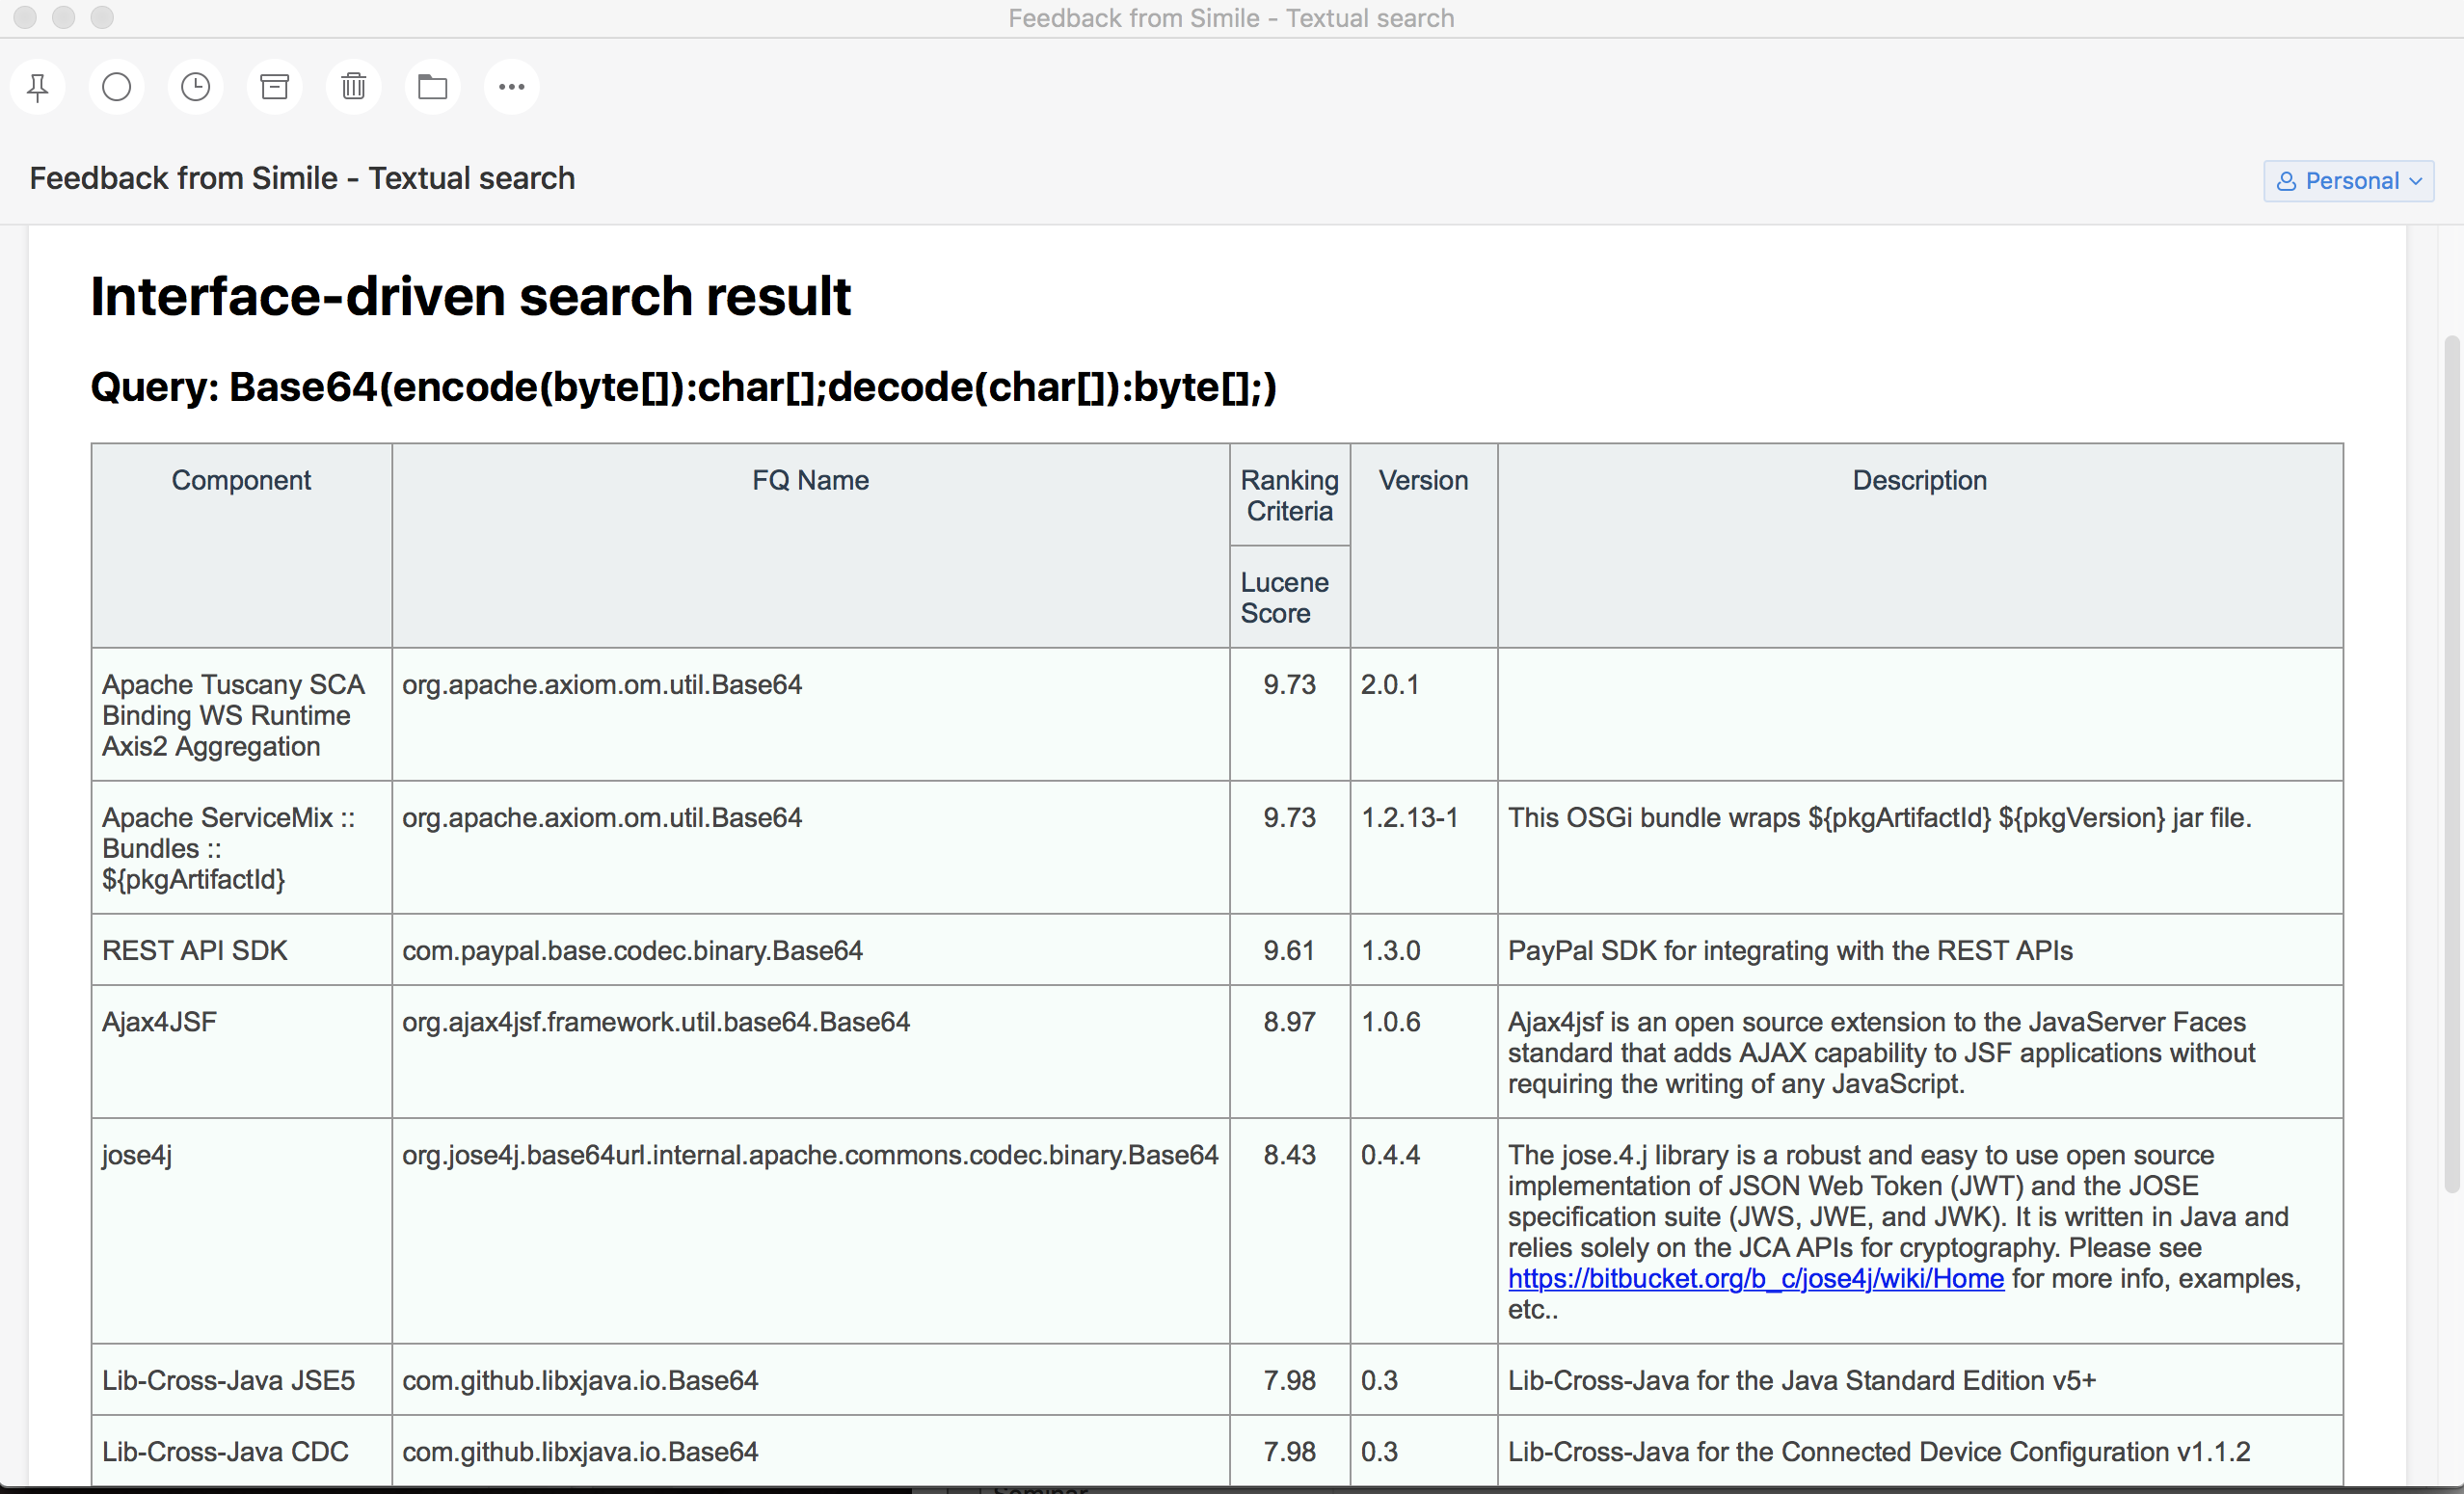
\includegraphics[width=0.7\textwidth]{grafiken/email-01}
    \caption{Textual search result email}
    \label{fig:email-01}
\end{figure}

\begin{figure}[H]
	\centering
    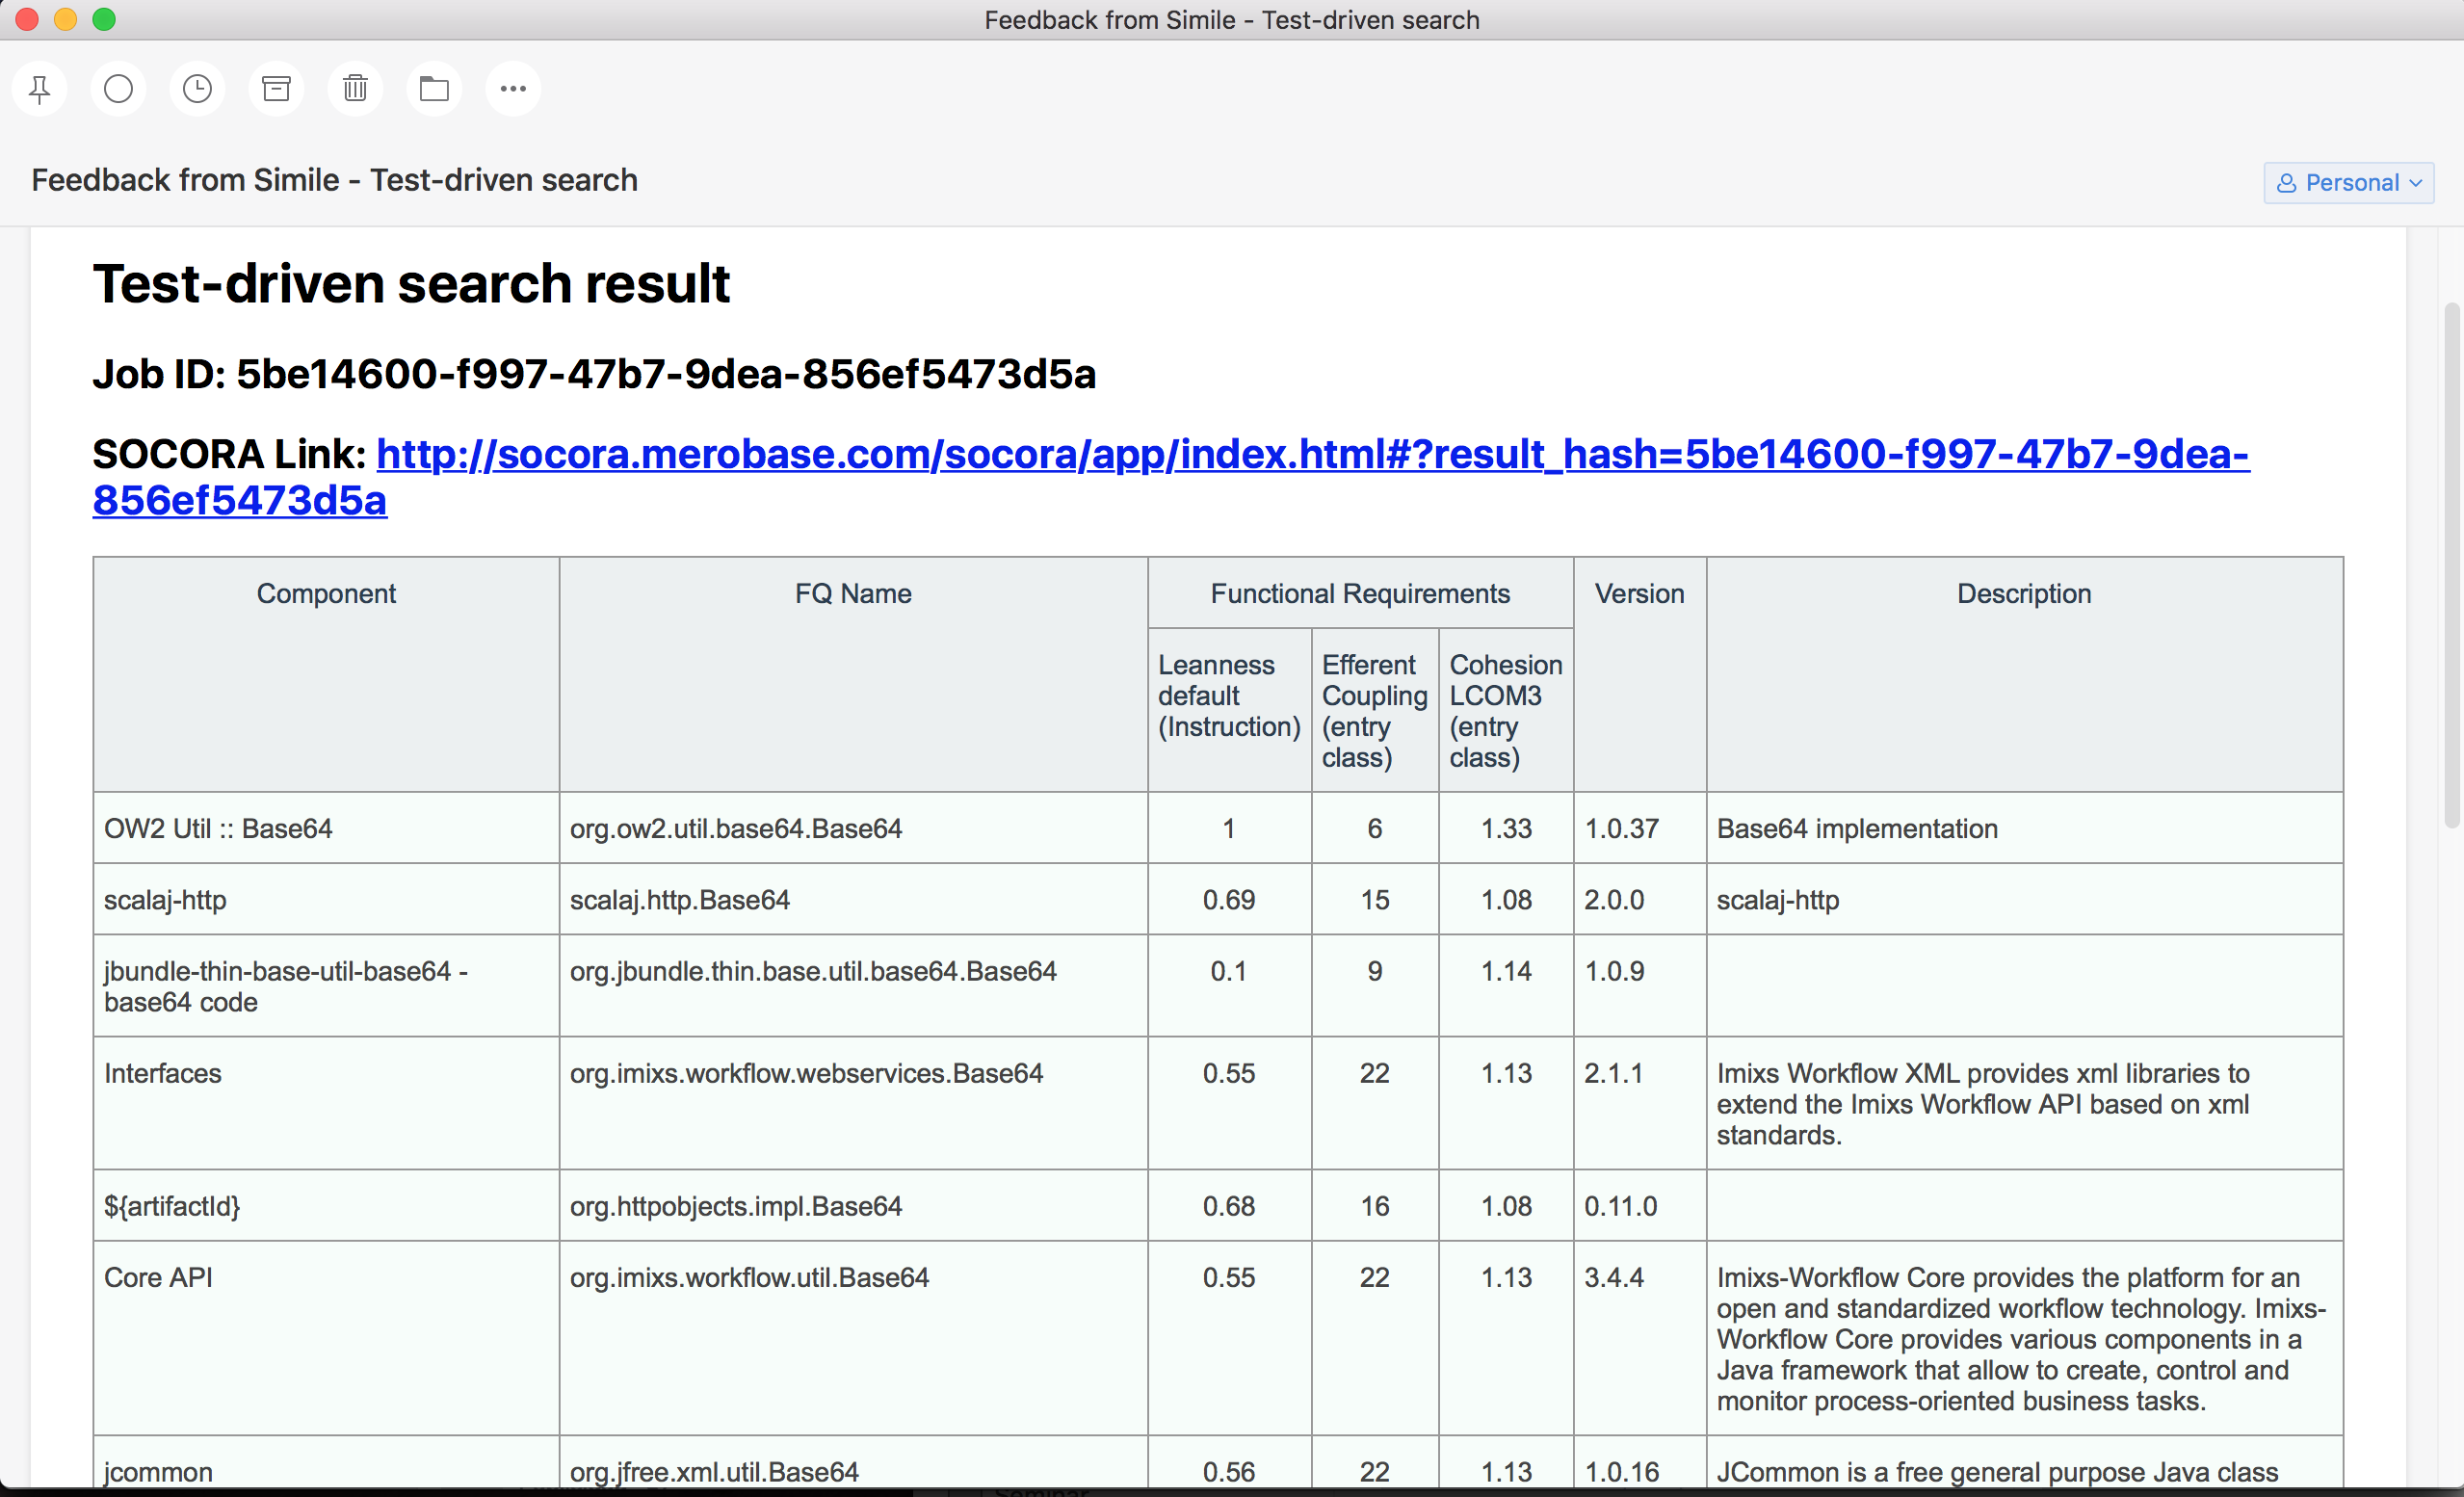
\includegraphics[width=0.7\textwidth]{grafiken/email-02}
    \caption{Test-driven search result email}
    \label{fig:email-02}
\end{figure}

Depending on the type of search, the email will have some differences. The text driven search result contains a the query sent to SOCORA and a table with the candidates found. For test-driven search result, the email contains the job id of the search, the link to SOCORA to see more details of the result and the list of candidates found.

\subsection{HTTP Controller}
The Java class EntryController.java [\ref{EntryController.java}] is in charge of receiving the request from a customer with the Git repository and the branch of the project to be analysed, and the email where the result of the similar component will be sent. In the listing \ref{setupRepository} we can see the method setupRepository which represents the entry point which is a POST request with the three parameters described before. The parameter \emph{repo} is required and represent the Git repository of the project that will be analysed and to which similar components will be searched for. The parameter \emph{branch} represents the branch of the git repository, this parameter is optional. Finally, the parameter \emph{email} represents the email where the result of the similar components will be sent to.

\lstinputlisting[
  language=Java, numbers=left, firstnumber=1, breaklines=true, 
  basicstyle=\footnotesize,
  numberstyle=\tiny,
  caption={Method setupRepository of EntryController.java},
  captionpos=b,
  label=setupRepository
]
{code/EntryController-setupRepository.txt}

When a request is received by the controller, it firstly validates if the parameters are correct. If they are not valid, it will respond with HTTP status code 400 and a message describing the errors. Otherwise, it triggers asynchronously the method searchForComponents with the repository, the branch, and a random CUID \footnote{CUID: Collision-resistant ids - \url{https://github.com/graphcool/cuid-java} (accessed: 04.02.2017).} as a folder name of the service Simile. This service is in charge of starting the process of cloning the project, analyse the code, make the request to SOCORA, and to send the email with the result to the customer.

\section{CI integration}
To integrate our prototype to a Continuous Integration process we decided to create a plugin. We decided to create our main prototype as independent as possible thus we do not depend on any CI tool. Therefore in this work to prove our approach we built a plugin for the CI server Jenkins. We decided to use Jenkins because is one of the most popular CI server for Java projects \footnote{\url{https://www.cloudbees.com/sites/default/files/2016-jenkins-community-survey-responses.pdf} (accessed: 04.02.2017)} and it is open-source.

The Simile Jenkins plugin is simple. First when a user creates a job in Jenkins, he/she can add a post build step. There he/she select the Simile plugin. When it is done, a new section is added in the task configuration (figure \ref{}). There he/she should add the Git repository of the project, the branch (optional), and the email. Once done, whenever the job is triggered, the plugin will be triggered too. The plugin sends via HTTP POST request the repository, branch, and email to Simile.

% ADD IMAGE OF JENKINS

In the future if Simile needs to be integrated to another CI server, we just need to develop a simple plugin which sends the information needed to look for similar components. 